\section{The Data}

\begin{frame}{Dataset Structure and Feature Groups}
	\begin{itemize}
		\item Sample size: about 26,707 respondents, with 35 predictors plus respondent identifier.
		\item Predictor groups:
		\begin{itemize}
			\item Behavioral actions (e.g., mask use, handwashing, avoidance)
			\item Attitudes and risk beliefs (e.g., concern, perceived vaccine effectiveness)
			\item Access and context (e.g., doctor recommendation, insurance)
			\item Demographics and geography (age, education, region, employment)
		\end{itemize}
		\item Mixed data types: binary, ordinal, nominal categorical, and count variables.
	\end{itemize}
\end{frame}

\begin{frame}{Planned Preprocessing and Validation Strategy}
	\begin{itemize}
		\item Missing data plan:
		\begin{itemize}
			\item Use explicit missing-category treatment for key categorical fields.
			\item Use structured imputation for selected predictors where justified.
		\end{itemize}
		\item Encoding plan:
		\begin{itemize}
			\item Keep ordinal scales ordered where meaningful.
			\item Use indicator encoding for nominal categories.
		\end{itemize}
		\item Evaluation split plan:
		\begin{itemize}
			\item Stratified cross-validation on both outcomes for robust model comparison.
			\item Report macro ROC AUC and probability calibration diagnostics.
		\end{itemize}
	\end{itemize}
\end{frame}

\begin{frame}{H1N1 Exploratory Data Analysis}
	\vspace{-1.75em}
	\begin{center}
		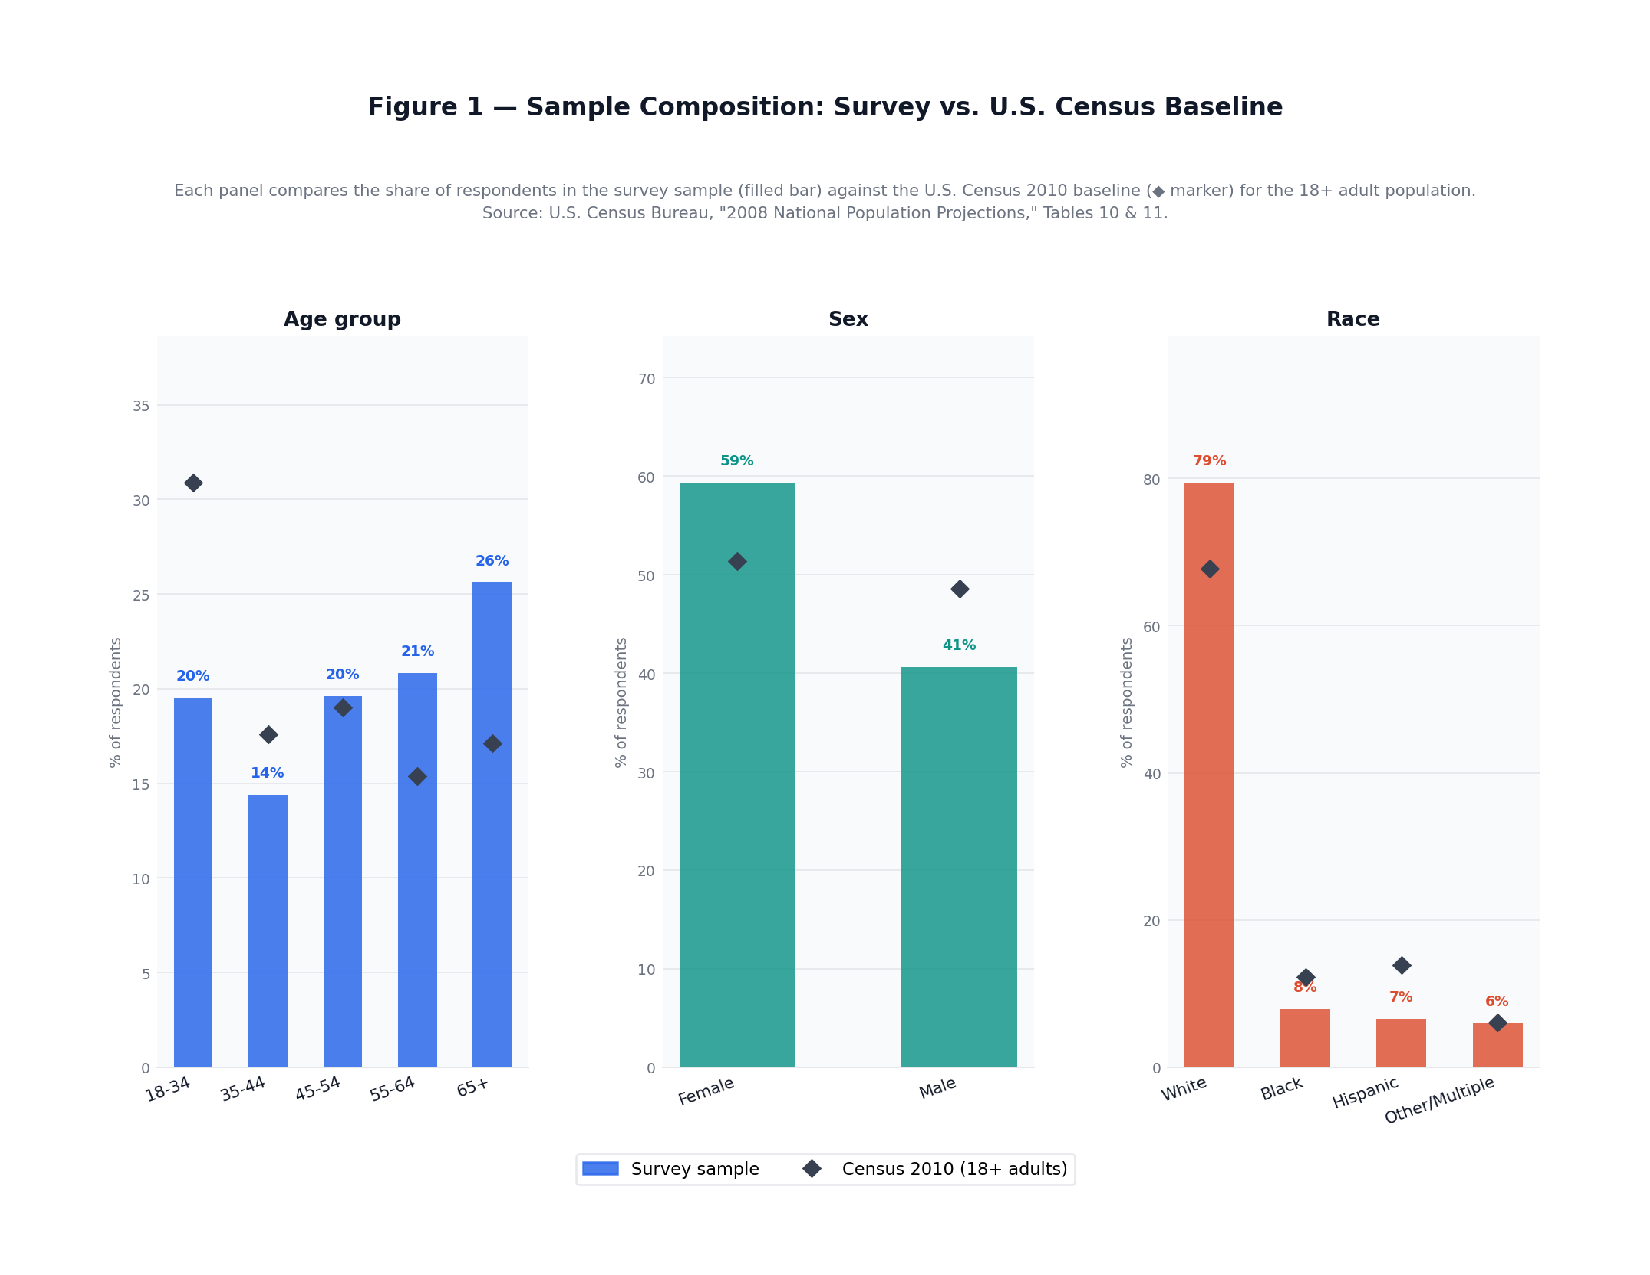
\includegraphics[height=1\textheight]{h1n1_eda_fig1.pdf}
	\end{center}
\end{frame}

\begin{frame}{H1N1 Feature Relationships}
	\vspace{-1.75em}
	\begin{center}
		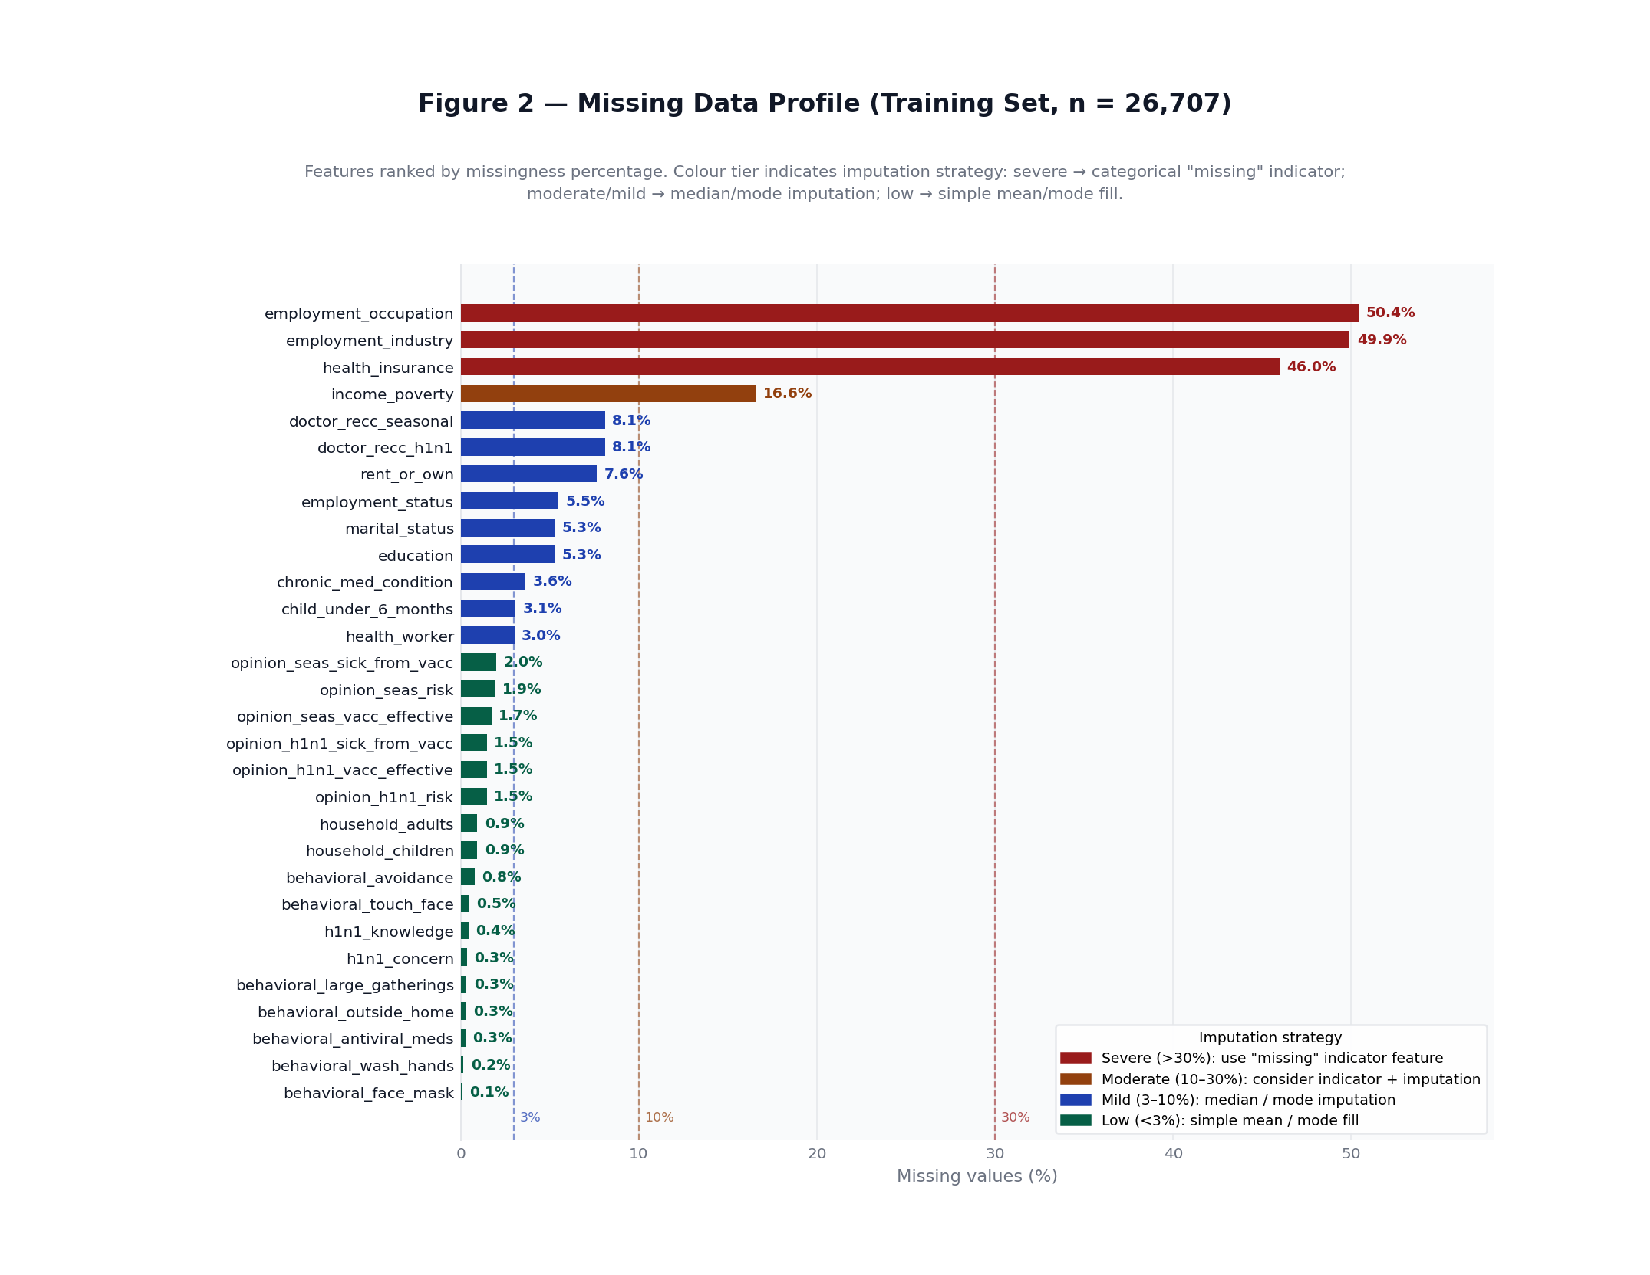
\includegraphics[height=1\textheight]{h1n1_eda_fig2.pdf}
	\end{center}
\end{frame}